\documentclass[10pt]{beamer}

\usetheme{CambridgeUS}
\usepackage[english, russian]{babel}
\usepackage[utf8]{inputenc}
\usepackage{caption}
\usepackage{etoolbox}
\usepackage{multicol}
\usepackage{listings}
\usepackage{wasysym}
\usepackage{mathtools}
\DeclarePairedDelimiter\ceil{\lceil}{\rceil}
\DeclarePairedDelimiter\floor{\lfloor}{\rfloor}

\definecolor{mygreen}{rgb}{0,0.6,0}
\lstset{
  basicstyle=\ttfamily\footnotesize,        % the size of the fonts that are used for the code
  breaklines=true,                 % automatic line breaking only at whitespace
  captionpos=b,                    % sets the caption-position to bottom
  commentstyle=\color{mygreen},    % comment style
  keywordstyle=\color{blue},       % keyword style
  stringstyle=\color{red},     % string literal style
  showstringspaces=false,
  morekeywords={include, printf},
  texcl=true     %<---- added
}


\title[\href{https://goo.gl/NRgp8K}{https://goo.gl/NRgp8K} (Term 1)]{Хеш-таблица. Открытая адресация}
\author[Гусев Илья, Булгаков Илья]{Гусев Илья, Булгаков Илья}
\institute[МФТИ] 
{Московский физико-технический институт\\*}
\date{Москва, 2018}
\subject{Computer Science}

\begin{document}

\begin{frame}
  \titlepage
\end{frame}

\begin{frame}{Содержание}
\tableofcontents
\end{frame}

\subsection{Открытая адресация}

\begin{frame}[fragile]{Открытая адресация}
\begin{center}
    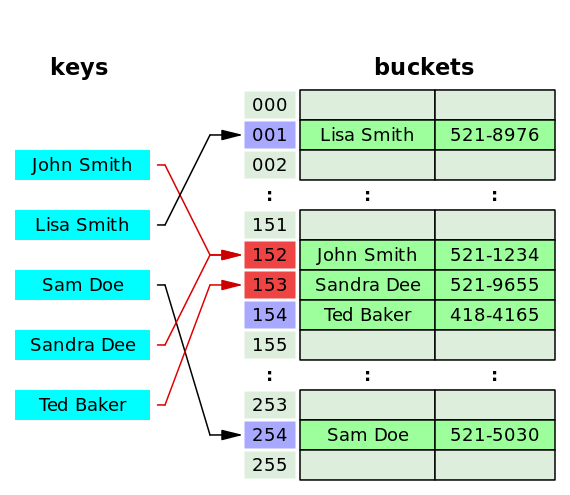
\includegraphics[width=10cm, height=7.7cm]{Term_1/Source/Pirctures/open.png}
\end{center}
\end{frame}

\begin{frame}[fragile]{Открытая адресация}
\begin{center}
    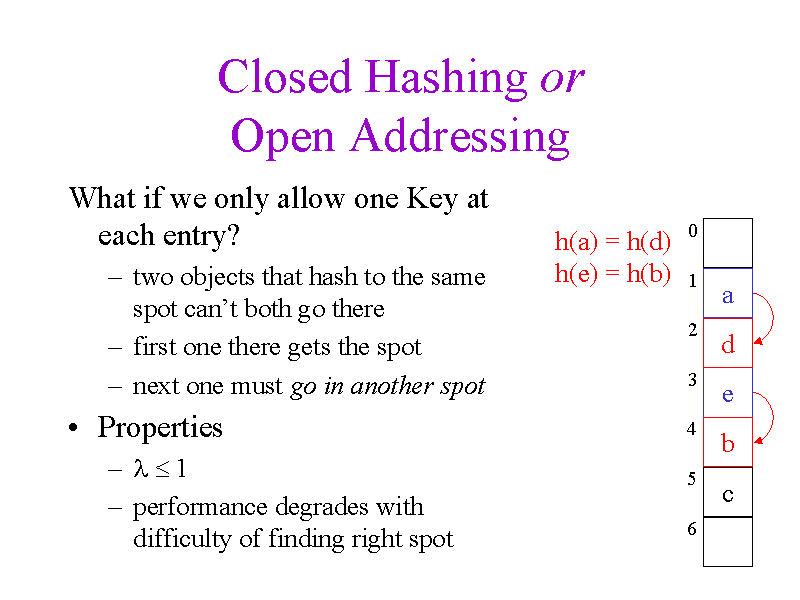
\includegraphics[width=10cm, height=7.7cm]{Term_1/Source/Pirctures/img012.png}
\end{center}
\end{frame}

\subsection{Методы пробирования}

\begin{frame}[fragile]{Методы пробирования}
В случае появления коллизий надо придумать, в каком порядке просматривать ячейки. Есть несколько подходов.
    \begin{itemize}
        \item Линейное пробирование \newline
            $H(k,i) = ( Hash(k) + i ) mod (m)$ 
        \item Квадратичное пробирование \newline
            $H(k,i) = ( Hash(k) + C1*i + C2*i^{2} ) mod (m)$ \newline
            Например, C1 = C2 = 1/2
        \item Двойное хеширование \newline
            $H(k,i) = ( Hash1(k) +i * Hash2(k) ) mod (m)$
    \end{itemize}
\end{frame}

\begin{frame}[fragile]{Линейное пробирование}
\begin{center}
    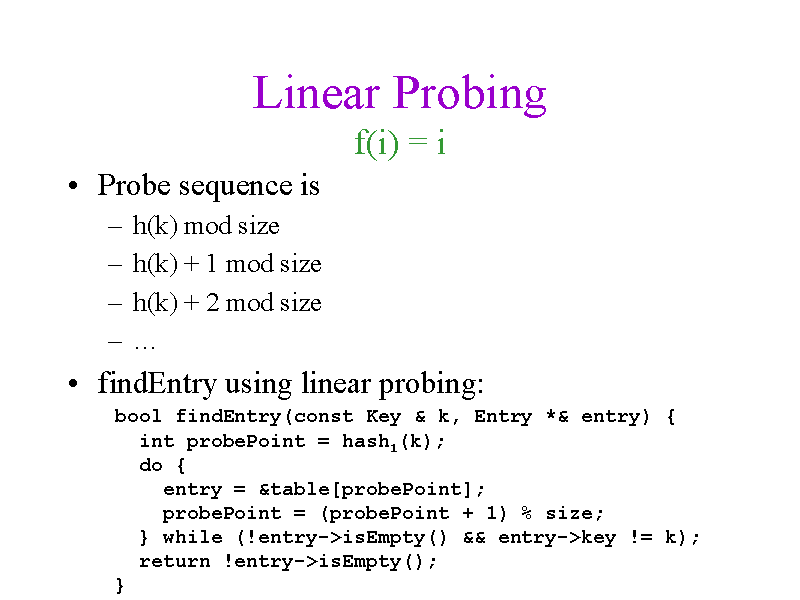
\includegraphics[width=10cm, height=7.7cm]{Term_1/Source/Pirctures/img014.png}
\end{center}
\end{frame}

\begin{frame}[fragile]{Линейное пробирование}
\begin{center}
    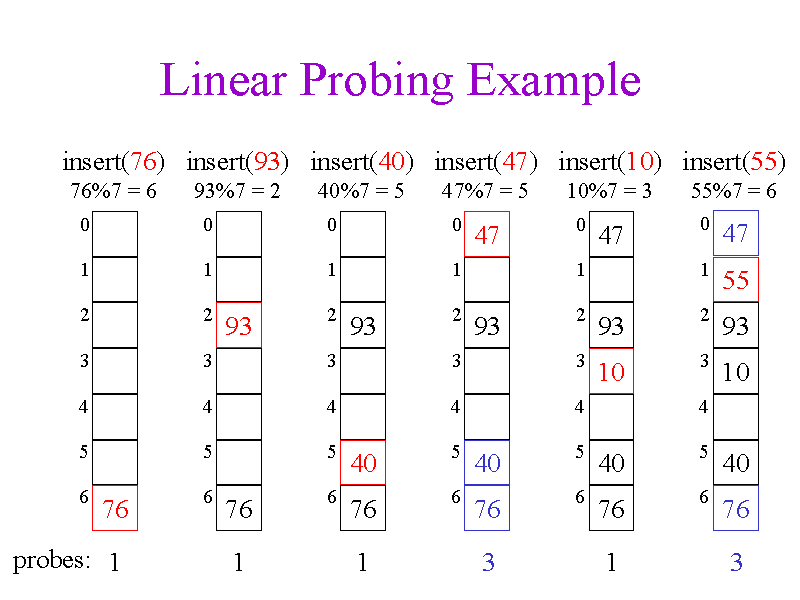
\includegraphics[width=10cm, height=7.7cm]{Term_1/Source/Pirctures/img015.png}
\end{center}
\end{frame}

\begin{frame}[fragile]{Квадратичное пробирование}
\begin{center}
    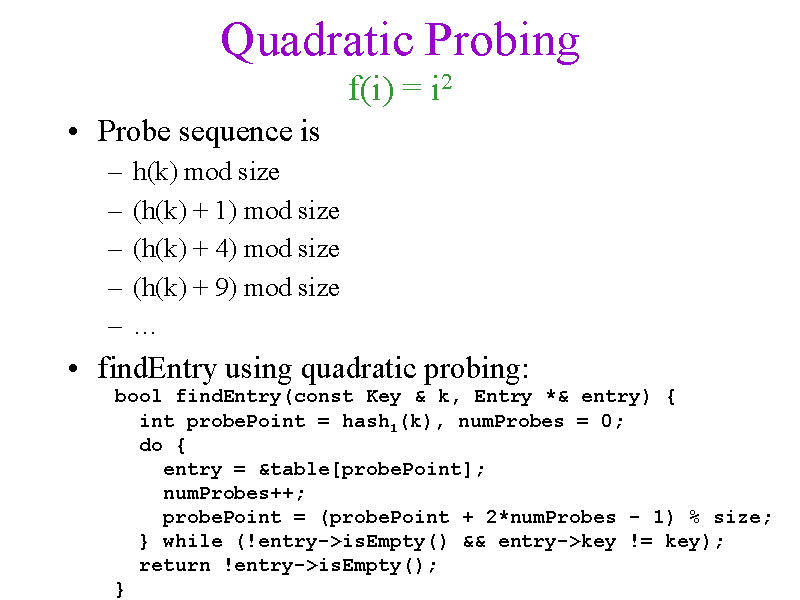
\includegraphics[width=10cm, height=7.7cm]{Term_1/Source/Pirctures/img017.png}
\end{center}
\end{frame}

\begin{frame}[fragile]{Квадратичное пробирование}
\begin{center}
    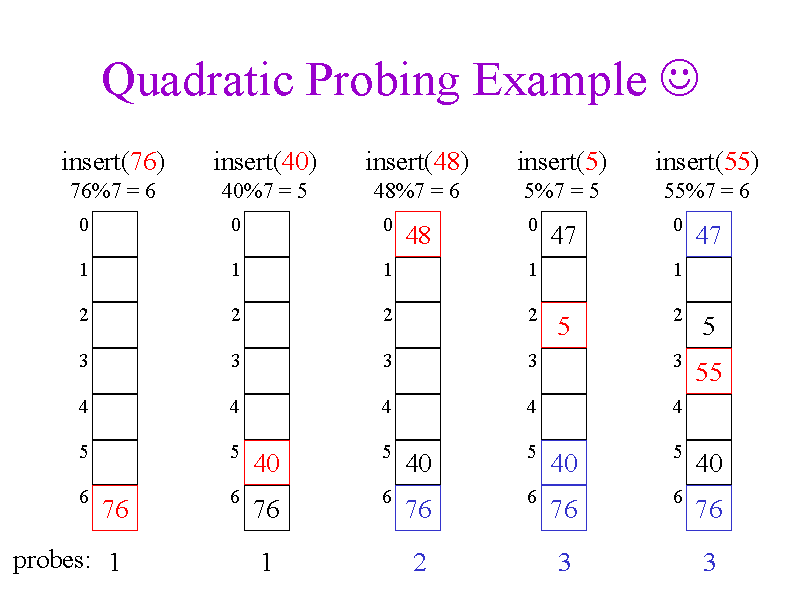
\includegraphics[width=10cm, height=7.7cm]{Term_1/Source/Pirctures/img018.png}
\end{center}
\end{frame}

\begin{frame}[fragile]{Квадратичное пробирование}
\begin{center}
    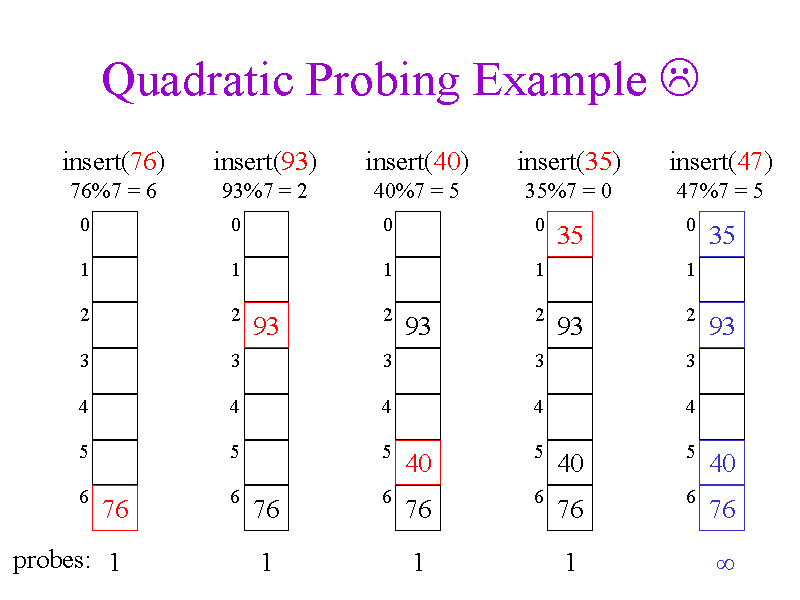
\includegraphics[width=10cm, height=7.7cm]{Term_1/Source/Pirctures/img019.png}
\end{center}
\end{frame}

\begin{frame}[fragile]{Двойное хеширование}
\begin{center}
    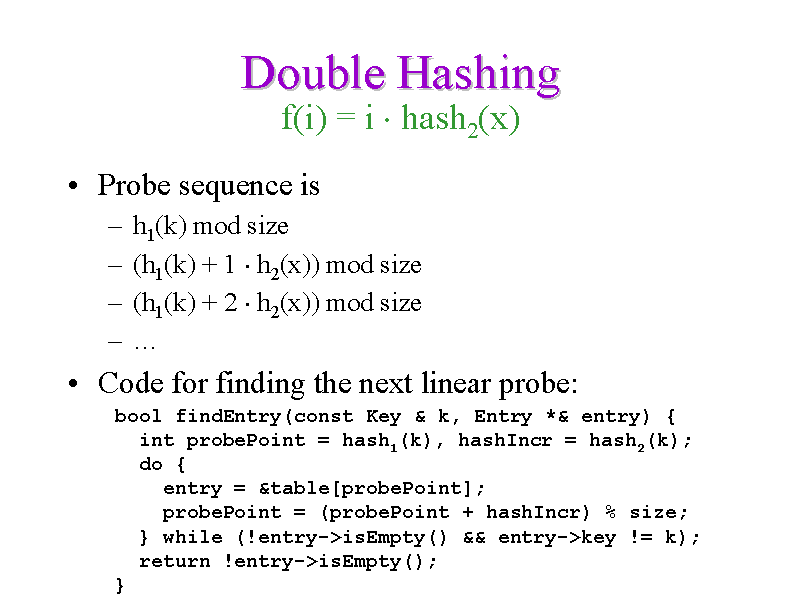
\includegraphics[width=10cm, height=7.7cm]{Term_1/Source/Pirctures/img023.png}
\end{center}
\end{frame}

\begin{frame}[fragile]{Двойное хеширование}
\begin{center}
    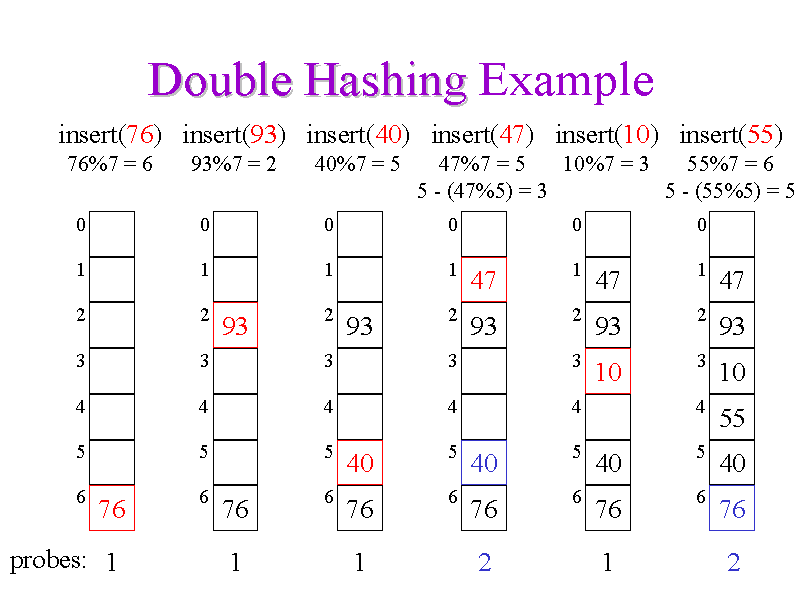
\includegraphics[width=10cm, height=7.7cm]{Term_1/Source/Pirctures/img025.png}
\end{center}
\end{frame}

\appendix

\section<presentation>*{\appendixname}
\subsection<presentation>*{Useful links}

\end{document}


